% ============================================================================
%  Rapport d'avancement — Simulateur V2V
%  Meryem Belmouaddine & Mohammed Chouadra — M1 IM/MIAGE
%  Encadrant : M. Moalic Laurent
%
%  Compilation :
%      pdflatex rapport.tex && pdflatex rapport.tex
% ============================================================================

\documentclass[a4paper,11pt]{article}

\usepackage[utf8]{inputenc}
\usepackage[T1]{fontenc}
\usepackage[french]{babel}
\usepackage{lmodern}
\usepackage{microtype}
\usepackage[a4paper,top=2.3cm,bottom=2.4cm,left=2.3cm,right=2.3cm]{geometry}
\usepackage{setspace}\setstretch{1.12}
\usepackage{parskip}
\usepackage{xcolor}

\definecolor{primary}{HTML}{0EA5E9}
\definecolor{primaryDark}{HTML}{0369A1}
\definecolor{accent}{HTML}{F59E0B}
\definecolor{ok}{HTML}{16A34A}
\definecolor{soft}{HTML}{F1F5F9}
\definecolor{rule}{HTML}{CBD5E1}

\usepackage[hidelinks,colorlinks=true,linkcolor=primaryDark,citecolor=primaryDark,urlcolor=primaryDark]{hyperref}

\usepackage{titlesec}
\titleformat{\section}
  {\Large\bfseries\color{primaryDark}}{\thesection.}{0.6em}{}
  [\vspace{-2pt}{\color{rule}\titlerule[0.5pt]}]
\titleformat{\subsection}
  {\large\bfseries\color{primary!85!black}}{\thesubsection}{0.6em}{}
\titlespacing*{\section}{0pt}{16pt}{6pt}
\titlespacing*{\subsection}{0pt}{10pt}{4pt}

\usepackage{fancyhdr}
\pagestyle{fancy}\fancyhf{}
\renewcommand{\headrulewidth}{0pt}
\fancyfoot[L]{\color{rule}\footnotesize Simulateur V2V — Rapport d'avancement}
\fancyfoot[R]{\color{rule}\footnotesize\thepage}

\usepackage{enumitem}
\setlist[itemize]{leftmargin=*,topsep=2pt,itemsep=2pt,parsep=0pt}

\usepackage{array}\usepackage{booktabs}\usepackage{tabularx}\usepackage{colortbl}

\usepackage{graphicx}
\graphicspath{{../IMAGES/}{figures/}}
\usepackage{caption}
\captionsetup{font=small,labelfont=bf,labelsep=period,labelfont={color=primaryDark}}

\usepackage[most]{tcolorbox}
\tcbset{
  card/.style={
    enhanced, colback=soft, colframe=primary!70,
    boxrule=0.4pt, arc=2.5pt, left=8pt,right=8pt,top=6pt,bottom=6pt,
    fonttitle=\bfseries, coltitle=primaryDark, title=#1
  },
  metric/.style={
    enhanced, colback=ok!10, colframe=ok!50,
    boxrule=0.4pt, arc=2.5pt, left=8pt,right=8pt,top=6pt,bottom=6pt
  }
}

\hypersetup{
  pdftitle  = {Simulateur V2V — Rapport d'avancement},
  pdfauthor = {Meryem Belmouaddine, Mohammed Chouadra}
}

\begin{document}

% --- Page de garde --------------------------------------------------------
\begin{titlepage}
\centering
\vspace*{1.2cm}


\includegraphics[height=3.2cm]{UHA_cartouche.png}

\vspace{1.8cm}
{\color{primaryDark}\rule{\linewidth}{1.5pt}}\vspace{0.4cm}

{\Huge\bfseries\color{primaryDark} Simulateur V2V}\\[6pt]
{\Large\bfseries Vehicle-to-Vehicle Communication}\\[10pt]
{\large\itshape Visualisation temps r\'eel d'un r\'eseau v\'ehiculaire intelligent\\
sur donn\'ees OpenStreetMap}\\[6pt]

{\color{primaryDark}\rule{\linewidth}{1.5pt}}

\vspace{1.8cm}\Large\bfseries Rapport d'avancement\\\normalsize\vspace{1.8cm}

\begin{tcolorbox}[card=Auteurs, width=10cm]\centering
{\Large Meryem \textsc{Belmouaddine}}\\[2pt]
{\Large Mohammed \textsc{Chouadra}}\\[4pt]
\textit{M1 IM/MIAGE}
\end{tcolorbox}\vspace{0.8cm}

\begin{tcolorbox}[card=Encadrement, width=10cm]\centering
M.~\textsc{Moalic} Laurent
\end{tcolorbox}

\vfill
{\color{rule}\rule{\linewidth}{0.4pt}}
{\small Ann\'ee universitaire 2025--2026}
\end{titlepage}

% --- Sommaire compact -----------------------------------------------------
{\color{primaryDark}\Large\bfseries Sommaire}\par\vspace{6pt}
{\color{rule}\hrule}\vspace{6pt}
{\small\setstretch{1.1}
\textbf{1.} Introduction \dotfill 2 \\
\textbf{2.} Architecture et choix techniques \dotfill 3 \\
\textbf{3.} \'Etat d'avancement par \'etape \dotfill 4 \\
\textbf{4.} D\'emonstration visuelle \dotfill 7 \\
\textbf{5.} R\'esultats de performance \dotfill 8 \\
\textbf{6.} Conclusion et perspectives \dotfill 9
}\par\vspace{8pt}
{\color{rule}\hrule}
\clearpage

% =========================================================================
\section{Introduction}

Les communications \textbf{V\'ehicule-\`a-V\'ehicule} (V2V) constituent une
brique fondamentale des syst\`emes de transport intelligents. Elles
permettent l'\'echange en temps r\'eel d'informations entre v\'ehicules
voisins : alertes d'accident, signalement de congestion, demandes de
priorit\'e pour les v\'ehicules d'urgence, etc. Leur d\'eploiement \`a grande
\'echelle d\'epend de la capacit\'e des algorithmes \`a passer \`a l'\'echelle
(milliers de v\'ehicules) et de la qualit\'e des mod\`eles de propagation
radio.

\subsection{Objectifs}

D\'evelopper en \texttt{C++20} un simulateur V2V offrant :

\begin{itemize}
\item visualisation temps r\'eel d'au moins 2\,000 v\'ehicules,
\item r\'eseau routier r\'eel import\'e depuis \textbf{OpenStreetMap},
\item d\'etection dynamique des liens V2V via une structure spatiale,
\item interface utilisateur compl\`ete pour piloter et observer la
      simulation,
\item architecture modulaire ouverte \`a des extensions ITS plus avanc\'ees.
\end{itemize}

\subsection{Synth\`ese d'avancement}

\begin{tcolorbox}[metric]
\centering\large
\textbf{14 \'etapes r\'ealis\'ees} \quad{\color{rule}\textbullet}\quad
\textbf{$\sim$ 5\,500 lignes de C++20} \quad{\color{rule}\textbullet}\quad
\textbf{19\,000 v\'ehicules} \\
simul\'es \`a \textbf{120 FPS} sur MacBook M2 (cible initiale~: 2\,000 v\'eh.\ @ 60 FPS)
\end{tcolorbox}

% =========================================================================
\section{Architecture et choix techniques}

\subsection{Pile technologique}

\begin{tcolorbox}[card=Stack]
\textbf{Langage :} C++20 (AppleClang).
\textbf{Graphique :} OpenGL 3.3 Core, GLFW 3.4 (fen\^etre + input), GLAD 2.0.6
(loader OpenGL), GLM 1.0.1 (alg\`ebre lin\'eaire), Dear ImGui 1.91.5
(interface).
\textbf{Donn\'ees cartographiques :} OpenStreetMap (tuiles CartoDB Voyager,
fichiers \texttt{.osm} XML via Overpass API), pugixml 1.14 (parsing XML),
stb\_image (PNG), libcurl (HTTP).
\textbf{Build :} CMake 3.20+ avec \texttt{FetchContent} pour toutes les
d\'ependances sauf libcurl (syst\`eme).
\end{tcolorbox}

\subsection{Organisation modulaire}

Le code est r\'eparti dans 8 sous-modules sans d\'ependance circulaire :

\begin{center}\small
\renewcommand{\arraystretch}{1.2}
\begin{tabularx}{\linewidth}{l X}
\toprule\rowcolor{soft}
\textbf{Module} & \textbf{R\^ole}\\
\midrule
\texttt{graphics/}   & Window GLFW, Camera2D pan/zoom, Shader, Renderer primitif\\
\texttt{map/}        & Projection Mercator EPSG:3857, TileCache LRU, TileLoader asynchrone\\
\texttt{graph/}      & RoadGraph (adjacency list), OSMParser XML, GraphRenderer\\
\texttt{simulation/} & Vehicle, VehiclePool, PathFinder A*, SimulationEngine, TrafficLightSystem, AccidentSystem\\
\texttt{v2v/}        & RadioModel, V2VNetwork, LinkRenderer, BroadcastSystem multi-hop\\
\texttt{ui/}         & ImGuiLayer (init RAII), panneaux ImGui en dashboard\\
\texttt{utils/}      & Profiler scop\'e, SpatialGrid uniforme, DensityHeatmap\\
\texttt{vendor/}     & TU pour stb\_image\\
\bottomrule
\end{tabularx}
\end{center}

\subsection{Boucle principale}

Chaque frame ex\'ecute, dans l'ordre :

\begin{enumerate}
\item Lecture des \'ev\'enements GLFW (souris, clavier).
\item \texttt{SimulationEngine::step(dt)} \textemdash{} avance tous les
      v\'ehicules, applique les feux et la collision avoidance.
\item \texttt{AccidentSystem::tick} \textemdash{} g\'en\'ere et g\`ere les
      \'epaves, d\'eclenche les alertes V2V.
\item \texttt{SpatialGrid} reconstruite, \texttt{V2VNetwork} d\'etecte les
      paires en port\'ee, \texttt{BroadcastSystem} fait propager les signaux.
\item Rendu monde : tuiles $\rightarrow$ heatmap densit\'e $\rightarrow$ graphe
      routier $\rightarrow$ v\'ehicules (instanced) $\rightarrow$ liens V2V
      $\rightarrow$ anneaux broadcast $\rightarrow$ marqueurs accidents.
\item Rendu UI : header dashboard + panneaux ImGui en tabs.
\end{enumerate}

% =========================================================================
\section{\'Etat d'avancement par \'etape}

Les 14 \'etapes du d\'eveloppement sont d\'ecrites de fa\c{c}on compacte ;
chacune produit un livrable ex\'ecutable.

\subsection*{\'Etape 1 — Fondations}

Structure des dossiers, \texttt{CMakeLists.txt} avec \texttt{FetchContent}
pour GLFW, GLM, GLAD~2, ImGui, pugixml et stb. Fen\^etre OpenGL~3.3 Core
fonctionnelle.

\subsection*{\'Etape 2 — Moteur graphique 2D}

\texttt{Window} (wrapper RAII de GLFW), \texttt{Shader} (compile / link /
cache d'\textit{uniforms}), \texttt{Camera2D} orthographique avec zoom
ancr\'e sur le curseur.

\subsection*{\'Etape 3 — Carte OpenStreetMap}

Projection Web Mercator (EPSG:3857), tuiles t\'el\'echarg\'ees en
\textbf{asynchrone} via libcurl (pool de 4 \emph{workers}), d\'ecodage PNG
hors thread GL, cache \textbf{LRU} born\'e \`a 512 tuiles, upload textures
c\^ot\'e thread principal.

\subsection*{\'Etape 4 — Graphe routier}

Parser pugixml du XML OSM, filtrage des \texttt{highway=*} routables.
Construction d'un graphe \textbf{dirig\'e} (\texttt{oneway} respect\'e,
\texttt{junction=roundabout} implicite). G\'eom\'etrie en
\textit{triangles \'epais} avec hi\'erarchie visuelle (motorway 16~m rouge
$\rightarrow$ service 4~m gris).

\subsection*{\'Etape 5 — Simulation des v\'ehicules}

\textbf{A* PathFinder} qui minimise le \textit{temps} de trajet (et non la
distance), heuristique admissible (euclidienne / $v_{\max}$). Buffers
r\'eutilis\'es entre appels via un \emph{compteur de g\'en\'eration} 32 bits
au lieu d'un reset $O(n)$. \textit{Random walk} non-U-turn comme fallback.

\subsection*{\'Etape 6 — Optimisation et observabilit\'e}

\textbf{Profiler scop\'e} (\texttt{V2V\_PROF("section")}) avec fen\^etre
glissante d'une seconde. \textbf{SpatialGrid uniforme} 500~m de c\^ot\'e \textemdash{}
\texttt{queryAllPairs(r)} en $O(n \cdot k)$ au lieu de $O(n^2)$.
\textbf{Rendu \emph{instanced}} des v\'ehicules : VBO statique de 3 vertices
(triangle unit\'e) + VBO dynamique d'instances ($N$ x position, heading,
couleur, taille) avec \texttt{glVertexAttribDivisor}.

\subsection*{\'Etape 7 — R\'eseau V2V}

\textbf{Mod\`ele radio} : $s(d, R) = 1 - (d/R)^2$ pour $d < R$. Port\'ee
effective $\min(R_a, R_b)$. \texttt{LinkRenderer} dessine tous les liens
en un seul \texttt{glDrawArrays(GL\_LINES)} color\'es selon la force
(rouge $\rightarrow$ jaune $\rightarrow$ vert).

\subsection*{\'Etape 8 — Interface Dear ImGui}

\texttt{ImGuiLayer} RAII autour des backends GLFW + OpenGL3. Sept panneaux
de pilotage : Controls, Layers, Simulation, V2V network, Performance,
Vehicle types, Selected vehicle.

\subsection*{\'Etape 9 — UX avanc\'ee}

Drag de la carte au clic gauche (avec d\'etection \emph{click vs drag} \`a 5
pixels de seuil), \textbf{taille de v\'ehicule adaptative} (clamp entre 14 et
100 pixels \'ecran), \textbf{s\'election d'un v\'ehicule} via
\texttt{SpatialGrid::queryRadius}.

\subsection*{\'Etape 10 — Types de v\'ehicules}

Cinq cat\'egories avec couleurs s\'emantiques :

\begin{center}\small
\begin{tabular}{lcccr}
\toprule\rowcolor{soft}
\textbf{Type} & \textbf{Couleur} & \textbf{Taille r\'eelle} & \textbf{$v_{\max}$} & \textbf{Part}\\\midrule
Car        & \cellcolor[HTML]{4DC7F4}\textcolor{white}{bleu ciel}   & 4{,}5 $\times$ 1{,}8 m & 130 km/h & 85 \%\\
Truck      & \cellcolor[HTML]{8C8F9F}\textcolor{white}{gris}        & 9{,}5 $\times$ 2{,}5 m & 90 km/h  & 7{,}5 \%\\
Bus        & \cellcolor[HTML]{F7C633}\textcolor{black}{jaune}       & 12 $\times$ 2{,}6 m    & 80 km/h  & 3 \%\\
Ambulance  & \cellcolor[HTML]{F5F5F5}\textcolor{black}{blanc}       & 5{,}8 $\times$ 2{,}2 m & 140 km/h & 2{,}5 \%$^{\dagger}$\\
Police     & \cellcolor[HTML]{4072FA}\textcolor{white}{bleu marine} & 4{,}8 $\times$ 1{,}9 m & 150 km/h & 2 \%$^{\dagger}$\\\bottomrule
\end{tabular}\\
{\footnotesize $^{\dagger}$ V\'ehicules d'urgence \textemdash{} port\'ee V2V augment\'ee de 150~m.}
\end{center}

\subsection*{\'Etape 11 — Comportement r\'ealiste}

\textbf{Anti-collision par-edge} : tri des v\'ehicules par progression sur
chaque ar\^ete, calcul de la distance bumper-\`a-bumper, ralentissement
lin\'eaire entre 5 et 20~m, arr\^et complet en de\c{c}\`a.
\textbf{Feux de circulation} : d\'etection automatique des intersections
(degr\'e $\geq 3$), cycles rond-robin de 7~s avec offset stagger\'e, arr\^et
\`a 93~\% de l'ar\^ete devant un feu rouge.
\textbf{Broadcast V2V multi-hop} : chaque v\'ehicule atteint par une onde
relaye automatiquement (jusqu'\`a 3 hops), couleurs distinctes par
g\'en\'eration (cyan $\rightarrow$ vert $\rightarrow$ jaune $\rightarrow$ orange).

\subsection*{\'Etape 12 — ITS avanc\'e}

\textbf{Heatmap de densit\'e} : grille 150~m avec smoothing temporel (demi-vie
0{,}7~s), gradient bleu $\rightarrow$ rouge.
\textbf{Accidents} : g\'en\'er\'es manuellement (touche \texttt{X}) ou
automatiquement sur d\'etection d'un \emph{tight-following} ; les v\'ehicules
impliqu\'es se figent comme obstacles ; un signal V2V d'urgence est
d\'eclench\'e automatiquement.
\textbf{Yielding aux v\'ehicules d'urgence} : tout civil dans un rayon de
45~m d'une ambulance/police voit son d\'ebit r\'eduit \`a 35~\% pendant
1{,}5~s.

\subsection*{\'Etape 13 — Inspecteur v\'ehicule intelligent}

T\'el\'em\'etrie \'etendue (distance parcourue, acc\'el\'eration, paquets
envoy\'es/re\c{c}us, temps de spawn) trait\'ee dans un panel \`a 11 sections :
\textit{Basic, GPS, V2V Communication, AI Decision Engine, Speed history,
Sensors, Network behaviour, Security \& Trust, Vehicle Health, Trajectory
Prediction, Recent Activity}. L'\textbf{AI Decision Engine} d\'erive la
d\'ecision actuelle (\textit{Cruising, Cautious follow, Stopped at red light,
Yielding, Hard braking}) et sa raison \`a partir de l'\'etat r\'eel.

\subsection*{\'Etape 14 — Dashboard professionnel}

Refonte de l'interface dans un style \textit{smart-transportation} :
th\`eme dark + accents n\'eon cyan, \textbf{header bar} avec stats globales
(VEHICLES / LINKS / FPS / AVG SIG / BROADCAST / ALERTS),
\textbf{Event feed} live des accidents, broadcasts et s\'elections,
inspecteur structur\'e en \textbf{tabs}
(\textit{Overview, Signals, Network, Sensors, AI, Security, Health}).

% =========================================================================
\section{D\'emonstration visuelle}

La figure~\ref{fig:overview} montre l'ensemble du syst\`eme en cours
d'ex\'ecution sur la zone urbaine de La~Rochelle (4\,000 v\'ehicules,
6\,800 liens V2V actifs).

\begin{figure}[!h]\centering
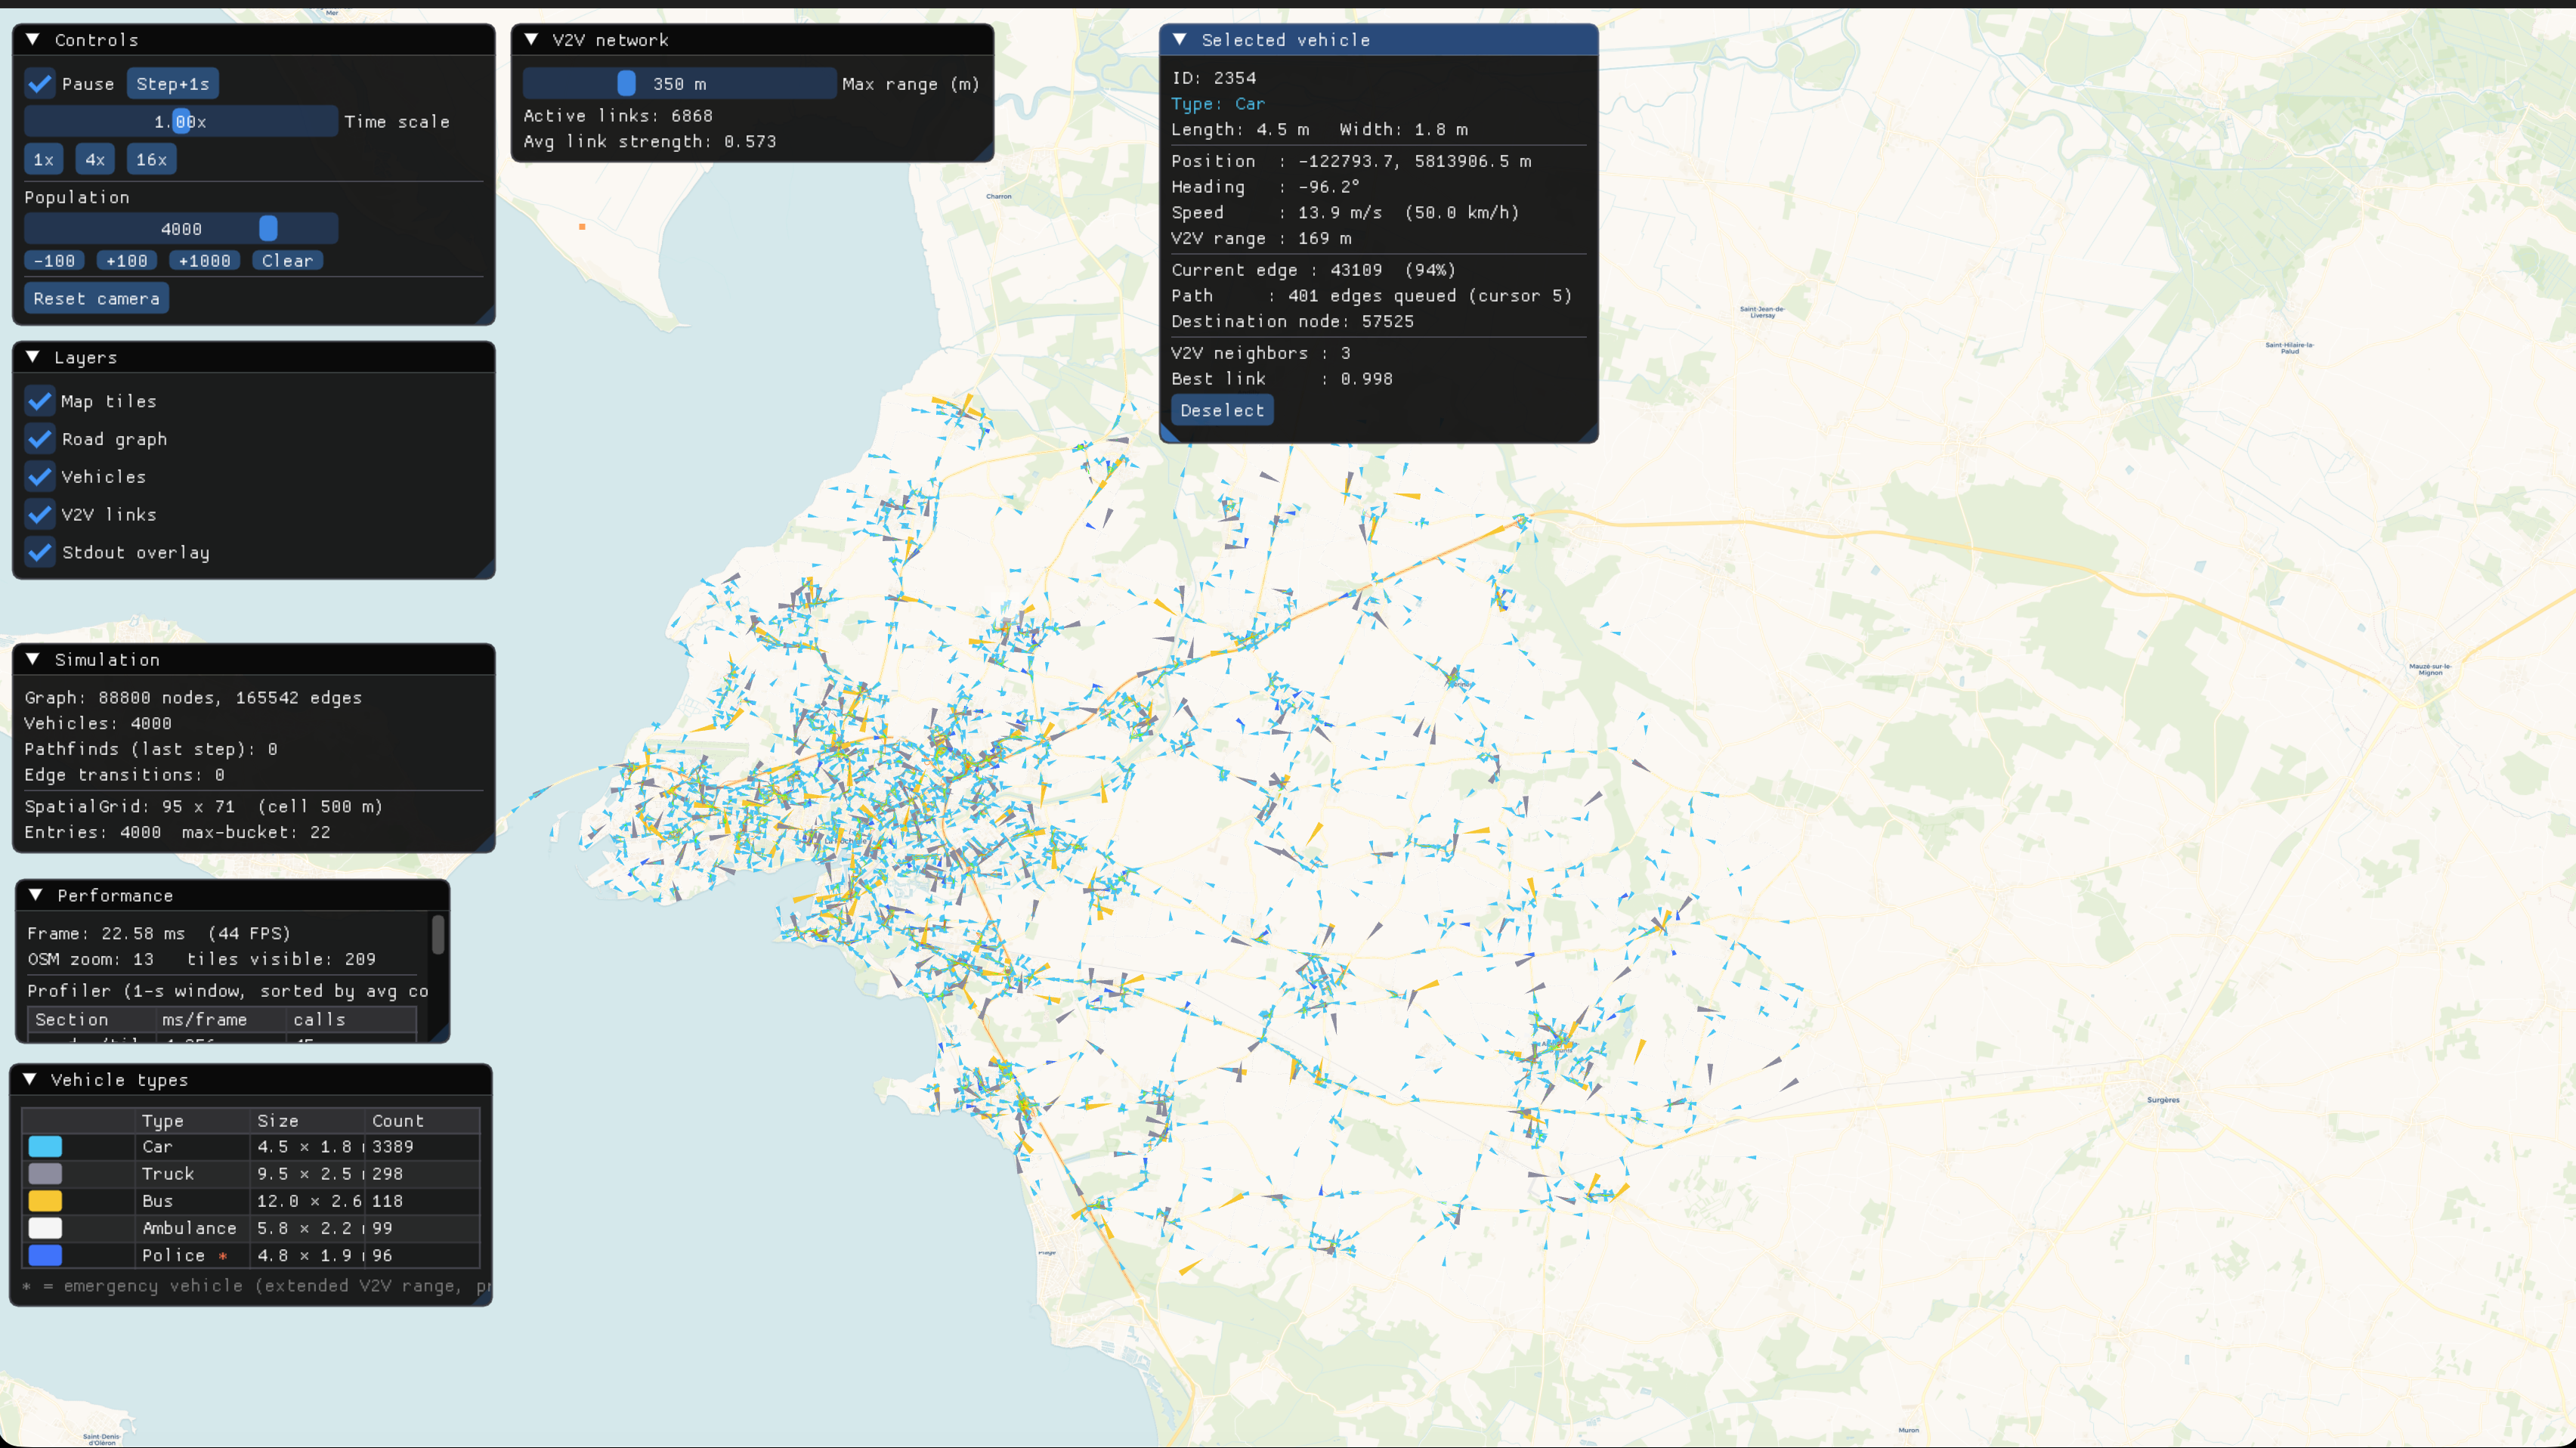
\includegraphics[width=\linewidth]{image.png}
\caption{Vue globale du simulateur \textemdash{} carte OpenStreetMap, graphe routier
hi\'erarchis\'e, $\sim$ 4\,000 v\'ehicules de 5 types diff\'erents avec leurs
liens V2V dynamiques, panneaux ImGui de contr\^ole et d'observation. Le
v\'ehicule s\'electionn\'e (Car \#2354) affiche son inspecteur complet en haut
\`a droite (3 voisins V2V, meilleur lien \`a force 0{,}998).}
\label{fig:overview}
\end{figure}

\textbf{\'El\'ements visibles sur la capture :}

\begin{itemize}
\item \textbf{Panneaux gauche} : Controls (pause, time scale, population
      4\,000), Layers (toggles), Simulation (graphe 88\,800 nodes / 165\,542
      edges, SpatialGrid 95$\times$71), Performance (44 FPS, profiler).
\item \textbf{Panneau central V2V} : 6\,868 liens actifs avec force moyenne
      0{,}573, port\'ee max param\'etrable.
\item \textbf{Panneau de droite} : inspecteur du v\'ehicule s\'electionn\'e
      (position, heading, vitesse, edge courante, path A* avec 401 hops
      restants, voisins V2V).
\item \textbf{Panneau bas} : l\'egende des cinq types avec compteurs live
      (3\,389 voitures, 298 camions, 118 bus, 99 ambulances, 96 police).
\item \textbf{Sur la carte} : triangles color\'es par type, lignes V2V vertes
      reliant les voitures proches, graphe routier orange en surimpression.
\end{itemize}

% =========================================================================
\section{R\'esultats de performance}

Les mesures sont prises avec le \texttt{Profiler} int\'egr\'e, fen\^etre
glissante d'une seconde, sur MacBook Air M2 (mat\'eriel grand public).

\begin{center}\small
\renewcommand{\arraystretch}{1.3}
\begin{tabularx}{\linewidth}{l r r X}
\toprule\rowcolor{soft}
\textbf{Section} & \textbf{ms/frame} & \textbf{appels/s} & \textbf{Commentaire}\\\midrule
\texttt{sim/step}        & 0{,}76 & 120 & avance v\'ehicules, collision, feux\\
\texttt{spatial/rebuild} & 0{,}08 & 120 & insert de 19\,000 entr\'ees\\
\texttt{v2v/update}      & 2{,}09 & 120 & 59\,000 paires d\'etect\'ees\\
\texttt{render/tiles}    & 0{,}11 & 120 & 84 tuiles charg\'ees\\
\texttt{render/graph}    & 0{,}04 & 120 & 1 draw call, 165\,k ar\^etes\\
\texttt{render/vehicles} & 0{,}07 & 120 & 1 draw \emph{instanced}, 19\,000 instances\\
\texttt{render/links}    & 0{,}33 & 120 & GL\_LINES, 59\,000 segments\\
\texttt{render/imgui}    & 0{,}13 & 120 & 7 panneaux ouverts\\\midrule
\rowcolor{soft}\textbf{Total approx.} & \textbf{$\sim$3{,}6 ms} & & \textbf{120 FPS} (marge $>$ 10 ms sur vsync 8{,}3 ms)\\\bottomrule
\end{tabularx}
\end{center}

\begin{tcolorbox}[metric]
\centering
\textbf{La cible 2\,000 v\'ehicules @ 60 FPS est d\'epass\'ee d'un facteur $\sim$10}~:\\
la configuration test\'ee tient \textbf{19\,000 v\'ehicules @ 120 FPS}.
\end{tcolorbox}

% =========================================================================
\section{Conclusion et perspectives}

\subsection{Bilan}

Le simulateur atteint l'int\'egralit\'e des objectifs initiaux et au-del\`a~:

\begin{itemize}
\item visualisation temps r\'eel d'un r\'eseau routier r\'eel OSM,
\item simulation de \textbf{19\,000 v\'ehicules} (objectif initial : 2\,000)
      \`a \textbf{120 FPS},
\item d\'etection dynamique des liens V2V via SpatialGrid en $O(n \cdot k)$,
\item gestion intelligente du trafic : anti-collision, feux de circulation,
      \textbf{accidents avec alerte V2V automatique}, broadcast multi-hop,
      yielding aux v\'ehicules d'urgence,
\item interface professionnelle type \textit{smart-transportation dashboard}
      (header + tabs + event feed + heatmap densit\'e),
\item code modulaire \texttt{C++20}, $\sim$ 5\,500 lignes, sans d\'ependance
      circulaire.
\end{itemize}

\subsection{Perspectives}

\begin{center}\small
\renewcommand{\arraystretch}{1.3}
\begin{tabularx}{\linewidth}{>{\color{primaryDark}\bfseries}c X}
\toprule\rowcolor{soft}
\'Etape & \textbf{Extension envisag\'ee}\\\midrule
15 & Communication V\'ehicule-Infrastructure (V2I) avec capteurs roadside
     et coordination des feux selon le trafic\\
16 & Tableau de bord r\'eseau (latence, taux de perte, paquets/s) bas\'e
     sur les compteurs r\'eels d\'ej\`a expos\'es\\
17 & M\'et\'eo (pluie, brouillard) impactant la port\'ee radio et la vitesse\\
18 & Syst\`eme de replay : enregistrement et rejeu d'une simulation\\
19 & Cybers\'ecurit\'e : v\'ehicules malveillants, d\'etection de paquets
     falsifi\'es (le \emph{Trust Score} simul\'e par l'inspecteur peut servir
     de base)\\
20 & Comportements autonomes : platooning, \'evitement d'obstacles, freinage
     d'urgence coop\'eratif\\\bottomrule
\end{tabularx}
\end{center}

\subsection{Comp\'etences mises en \oe uvre}

\textbf{C++ moderne} (C++20, RAII, templates, \texttt{std::function},
multithreading l\'eger). \textbf{Graphique} : OpenGL 3.3 Core, GLSL,
\emph{instancing}. \textbf{Algorithmique} : A*, graphe adjacency list,
\emph{uniform grid} spatial. \textbf{R\'eseau} : pool de \textit{workers}
threads, \texttt{std::mutex}, condition variables. \textbf{Cartographie} :
projection Web Mercator EPSG:3857. \textbf{Build} : CMake moderne avec
\texttt{FetchContent}. \textbf{UI} : Dear ImGui, layout dashboard.

\end{document}
